\documentclass[]{article}
\usepackage{cite}
\usepackage{hyperref}
\usepackage{multicol}
\usepackage{graphicx}

\graphicspath{ {images/} }
\setlength{\parskip}{0.5em}

\begin{document}

\begin{titlepage}
    \begin{center}
        \vspace*{1cm}
        
        \Huge
        \textbf{Using WordNet and Short-Term Memory for Contextual Disambiguation}
        \vspace{2cm}
        
        \Large
        \textbf{William T. F. Strachan}
        
        \vfill
                
        \vspace{0.8cm}
        
        \Large
        Word Count - PLACEHOLDER\\
        Supervisor - Dr Dimitar Kazakov\\
        Department of Computer Science\\
        University of York\\
        20 November 2016
        
    \end{center}
\end{titlepage}

\tableofcontents

\newpage
% ------------------------------ START OF DISSERTATION ------------------------------

\section{Literature Review}
\label{sec:LitReview}
In order to define a problem, we must first establish the previous works, so as to build upon them effectively. 
		
%--------------------- NLP

\subsection{Natural Language Processing}
\label{sec:NLP}
The study of natural language processing aims to allow a computer to understand natural language, and formulate a relevant response based upon its input. Within this, the problem of input text analysis has traditionally be broken down into smaller sub-problems\cite{NLPHandbook}:
\begin{itemize}
	\item Text Preprocessing
	\item Lexical Analysis
	\item Syntactic Parsing
	\item Semantic Analysis
\end{itemize}
The subsequent subsections will discuss each of these in more detail.

\subsubsection{Text Preprocessing}
\label{sec:TextPreprocessing}
Before any analysis can take place, the inputted raw text must be converted into a usable format. This, once again, can be broken down into multiple steps\cite{NLPHandbook}:
\begin{itemize}
	\item \textbf{Document Triage}

	\begin{itemize}
		\item Character encoding must be identified.
		\item The language can then be identified. %Language is most commonly found using one of two methods: Language can be identified by character set, in cases where language uses a unique alphabet, or by character frequency, in other cases.
		\item Non-useful data, such as images and html formatting must be removed.			\end{itemize}	
	\item \textbf{Text Segmentation}
	
	\begin{itemize}
		\item Individual words (tokens) must be separated from one another. % This is done using white space in space-delimited languages, and comprehensive lists in unsegemented languages
		\item Text Normalisation; replacing multiple equivalent tokens with one token (e.g. "Ave." and "Avenue").
		\item Identifying sentences, i.e. locating where a sentence begins and ends. 
	\end{itemize}
	
\end{itemize} 
% ########################
% #  UNFINISHED SECTION  #
% ########################


\subsubsection{Lexical Analysis}
\label{sec:LexicalAnalysis}
One word can have multiple forms, for example "judge" (the lemma) has the forms \{"judge", "judges", "judging", "judged"\} (morphological variants).  The job of Lexical Analysis is to replace all morphological variants of a word, with their corresponding lemma, a process known as stemming \cite{NLPHandbook}.

% In terms of ease of token identification, it can be seen conceptually how this process is beneficial. With that said, when we consider the amount of information in a word, it can similarly be realised that we lose information about the form of a word, for example plural/singular and tense.
\subsubsection{Syntactic Parsing}
\label{sec:SyntacticParsing}
Whwn derviving meaning from sentances, the grammatical structure can provide important insight. The Syntactic parsing technique extracts this infomation using two processes \cite{NLPAlmostFromScratch}: 
\begin{itemize}
	\item \textbf{Part-of-speech (PoS) Tagging}
	\label{PoSTag}
	\begin{itemize}
		\item Each word is given tags denoting their syntactic role (e.g. noun/adjective/verb).
	\end{itemize}		
	
	\item \textbf{Chunking}
	
	\begin{itemize}
		\item Noun phrases and verb phrases are detected and tagged using "begin chunk" and "inside chunk" labels
	\end{itemize}	
	
\end{itemize}

\subsubsection{Semantic Analysis}
\label{sec:SemanticAnalysis}
The semantics of a sentence, is the meaning given by it's tokens \cite{SemanticAnalysisAPracticalIntro}. The topic of semantic analysis will be expanded upon on in the \hyperref[sec:PrevWork]{Previous Works Section}.



%------------ Memory Models
\subsection{Psycholinguistics}
\label{sec:Psycholinguistics}
Language understanding is a problem which, it can be stated, is solved by the human brain. From this satatement, it can be derived that a computational solution could be effectively built around knowledge of the processes at work in the brain. The process of language comprehension can be described using the working memory model \cite{MemoryBaddeleyEysenkAnderson}.

According to Baddely et al. \cite{MemoryBaddeleyEysenkAnderson} there exist multiple, special purpose, memory structures within two main categories, the Short-term Store and the Long-term Store.  

\subsubsection{Long-term Store}
\label{LongTerm}
The long-term store (LTS) contains semi-permanent information. Within the LTS, there exist Explicit and Implicit memory structures. The contents of the Implicit memory describe skills and methods of doing things, whereas the Explicit memory contains factual information\cite{MemoryBaddeleyEysenkAnderson}. When considering these structures, it can be seen that Explicit memory is of greater interest in the context of NLP.

Within the Explicit memory exists knowledge of semantics \cite{MemoryBaddeleyEysenkAnderson}. The information held here not only defines concepts (meanings of word forms), but also their attributes and rules of use. In 1966, M. Quillain proposed a model of Semantic Memory \cite{SemanticMemoryQuillain}. The model consists of a graph of nodes, each representing a concept, connected by edges of differing types, each representing a different syntactic feature (for example, hypernym). 


\subsubsection{Short-term Store}
\label{ShortTerm}
The short-term store (STS) is a structure of limited capacity, used to store items for periods usually of no more than a few seconds \cite{MemoryBaddeleyEysenkAnderson}. In 1955, G. Miller, based upon previous experimental results, concluded that the size of the STS existed in the realm of 7$\pm$2 items of information \cite{SevenPlusMinusTwo}. 

In 1971, R. Atkinson and R. Shiffrin proposed a model of the STS \cite{ControlProcessesSTMAtkinson}. In this model, the STS can both send information to, and draw information from the LTS. Inputs from the sensory registers (memory structures holding information relating to inputs from senses) are also sent to the STS. Atkinson and Shiffrin proposed that, over time, the activation of items in the STS decreased; they went on to theorise that items could be lost from the STS, only when a new, more highly activated item could take its place. To counter this loss of activation, the authors discussed the control process, rehearsal. This process makes use of repetition to increase the activation of items in memory, decreasing their chance of loss. 

\subsubsection{Disambiguation Models}
\label{sec:DisambiguationModels}
In some cases, when assigning meaning to words, ambiguity can arise. Some words have multiple concepts, for example, bank can refer to a building, or a sloped surface alongside a body of water. In such cases, the brain uses some process to select the correct concept. One such model of this disambiguation is the Multiple-access model \cite{PsychologyOfLanguage}.

According to the multiple-access model, when presented with an ambiguious word, initially all corresponding concepts are activated \cite{AccessingLexicalAmbiguities}. The most appropriate concept is then chosen using context and frequency.

Previously, we established that the process of disambiguation begins with the activation of all possible word concepts. The context-sensitive model deals with the use of context and frequency in the selection of the most appropriate of these \cite{PsychologyOfLanguage}. In cases where the context is strong, i.e. the correct concept can be chosen using it's surrounding context, the context is primarily relied upon for disambiguation. In the opposite case, i.e. when context gives little indication of which is the correct concept, the most frequenly used concept is used, assuming it fits with the available context.


%------------ WORDNET
\subsection{Wordnet}
\label{Wordnet}
In 1990, it was noted by G. Miller et al. that current attemps to organise the english lexicon, i.e. conventional dictionaries, offered few benefits when used in conjunction with computers \cite{WN1Introduction}. Wordnet was an effort to produce a dictonary, containing more information than a conventional dictionary, that could be useful for computational applications.

\label{Synsets}Central to the design of wordnet, is the idea of synsets \cite{WN1Introduction}. The authors began using the assumption that all concepts can be uniquely defined by their set of synonyms (words which share like meaning). In most cases, this assumption holds true, though, in cases where more detail is required, a "gloss" was added \cite{WN1Introduction}.

Wordnet builds upon models of the semantic memory, such as that discussed in the \hyperref[LongTerm]{Long-term store section} \cite{WN1Introduction}. The overall structure relies on four main semantic relations:

\begin{itemize}
	\item Synonymy
	\begin{itemize}
		\item If two words are to be called synonyms, they must share at least one like meaning.
	\end{itemize}
	
	\item Atonymy \label{Atonym}
	\begin{itemize}
		\item Conceptually, Atonymy can be seen as the opposite of Synonymy. Atonymy is difficult to define, as not all words which share opposite meaning can be called atonyms, for example, \{up, down\} is an atonym pair, but \{up, fall\} is not.
	\end{itemize}
	
	\item Hyponymy
	\begin{itemize}
		\item If we consider a a synset to be a object-oriented class, its hypernym can be considered its parent class, for example, birch is a type of tree.
	\end{itemize}
	
	\item Meronymy \label{Meronym}
	\begin{itemize}
		\item Meronymy is relationship between two synsets where one is a part of another, for example, a goat has horns, therefore horn is a meronym of goat.
	\end{itemize}
	
\end{itemize}

It is common knowledge that words can fall into one of a number of categories, nouns, adjectives, verbs and adverbs. G. Miller et al. note that, due to the differences in the relations between words in these categories, each type has differs in the structure they produce and are therefore held in different files \cite{WN1Introduction}. The proceeding subsections will go into each of thesecategories in more detail.

\subsubsection{Nouns}
\label{Nouns}
G. Miller et al. note that a noun can be defined using only its immediate hypernym, and how it differs from its hypernyms other hyponyms \cite{WN2Nouns}. From this, it can be seen that hyponymy is perhaps the most important relation in the organisation of nouns. For this reason, nouns form a hierachical structure in wordnet.

Wordnet's designers stated the assumption that all nouns can be contained in a single hierachial structure \cite{WN2Nouns}. The issue with having a single word, of which all other words are hyponyms, is that this hypernym is relatively meaningless. It was instead decide to divide all words into 25 separate files, each containing a hierachical tree beginning with one of the following synsets \cite{WN2Nouns}:

\begin{multicols}{2}
\begin{itemize}
	\item[] \{act, action, activity\}
	\item[] \{animal, fauna\}
	\item[] \{artifact\}
	\item[] \{attribute, property\}
	\item[] \{body, corpus\}
	\item[] \{cognition, knowledge\}
	\item[] \{communication\}
	\item[] \{event, happening\}
	\item[] \{feeling, emotion\}
	\item[] \{food\}
	\item[] \{group, collection\}
	\item[] \{location, place\}
	\item[] \{motive\}
	\item[] \{natural object\}
	\item[] \{natural phenomenon\}
	\item[] \{person, human being\}
	\item[] \{plant, flora\}
	\item[] \{possession\}
	\item[] \{process\}
	\item[] \{quantity, amount\}
	\item[] \{relation\}
	\item[] \{shape\}
	\item[] \{state, condition\}
	\item[] \{substance\}
	\item[] \{time\}
\end{itemize}
\end{multicols}

Other than synonymy, nouns have three other important features \cite{WN2Nouns}:
\begin{itemize}
	\item Attributes
	\begin{itemize}
		\item The attributes of a noun consist of adjectives which distinguish it from other hyponyms of its hypernym, for example \{huge, green, fluffy\}.
	\end{itemize}		
	
	\item Parts
	\begin{itemize}
		\item The parts of a noun consist of its meronyms, described \hyperref[Meronym]{previously}.
	\end{itemize}		
	
	\item Functions
	\begin{itemize}
		\item The functions of a noun consist of verbs which are associated with its actions, for example chair has the functions \{sit, rest\}.
	\end{itemize}		
	
\end{itemize}

\subsubsection{Adjectives}
\label{Adjectives}
Adjectives in can be divided into four distinct groups, each implying a different structure of semantic links \cite{WN3Adjectives}:
\begin{itemize}
	\item Descriptive Adjectives
	\begin{itemize}
		\item As stated in the \hyperref[Nouns]{previous section}, nouns have attributes. Descriptive adjectives act as modifiers for these attributes: for example, a building has a height, by saying "tall building", the height attribute is given a value \cite{WN3Adjectives}. Atonymy, defined \hyperref[Atonym]{previously}, is considered by wordnet's designers to be the most important relation between descriptive adjectives. Unfortuantely, not all adjectives have atonyms, leading to the designer's addition of an indirect antonym" semantic link, between synonyms of a word and its atonym \cite{WN3Adjectives}. These semantic links give rise to a structure made up of pairs, linked to one another by their synonyms.
	\end{itemize}		
		
	\item Reference-Modifying Adjectives
	\begin{itemize}
		\item Reference-modifying adjectives have an adverb form which can be used to convey the same meaning \cite{WN3Adjectives}. For example, the noun-phrase "the former manager", can be modified to become "the man who was formerly a manager", without diverging from its original meaning. There exist relatively few examples of this category, so no overarching structure emerges, that being said, in some cases, the atonym relation does occur \cite{WN3Adjectives}.
	\end{itemize}
	
	\item Colour Adjectives
	\begin{itemize}
		\item As their name suggests, colour adjctives concern the value of the colour attribute. This definition implies that these words should, in fact, fit into the descriptive adjective category. Their separation is given by colour adjectives lack of true atonym (excluding modifiers such as "light" and "dark") \cite{WN3Adjectives}. The lack of clear semantic relations between these words poses a problem for their organisation, leading wordnet's designers to link them using their definitions, i.e. using hue, lightness and saturation.
	\end{itemize}	
	
	\item Relational Adjectives
	\begin{itemize}
		\item In the phrase "maternal instinct", it can be seen that the adjective is derived from a noun, in this case "mother"; this is the defining feature of relational adjectives \cite{WN3Adjectives}. In wordnet, relational adjectives are linked to their noun form, meaning they don't posess their own structure, instead falling into that described in the \hyperref[Nouns]{Noun section}.
	\end{itemize}		
		
	
\end{itemize}


\subsubsection{Verbs}
\label{Verbs}
In C. Fellbaums 1990 paper, "English Verbs as a Semantic Net", she discussed the lack of true synonymy across the verb category \cite{WN4Verbs}. This is an issue for Wordnet's designers, with their reliance on \hyperref[Synsets]{synsets}. The author goes on to describe the solution, periphrases, the use of verb phrases to give more meaning to a simple verb. In the paper, the example synset, \{swim, travel through water\} was given. 

The relationships between verbs follow a hierachy shown in Figure \ref{fig:WN4Verbs_pp15}, with each type elaborated upon in the following paragraphs.

\begin{figure}[h]
	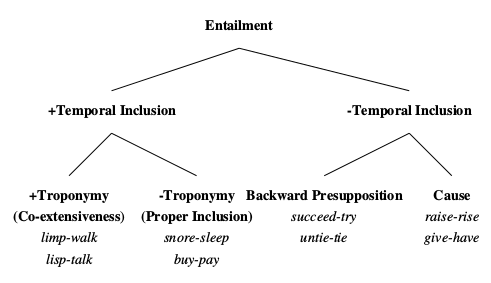
\includegraphics[scale=0.7]{WN4Verbs_pp15.png}
	\caption{HIERACHY OF SEMANTIC RELATIONS BETWEEN VERBS \cite[p.~15]{WN4Verbs}}
	\label{fig:WN4Verbs_pp15}
\end{figure}

\textbf{Entailment} is a relation, simlar in nature to hyponymy. A verb (a) is said to entail another (b) if, when b is substituted for a in a sentace, the truth value of the sentance remains the same \cite{WN4Verbs}. For example, "run" entails "move", "she ran" can also be described by "she moved". If a entails b, and b entials a, a and b are synonyms.

\textbf{Temporal Inclusion} is a form of entailment where one verb (a) is temporally included in another (b) if, b can only occur during the same time period as a\cite{WN4Verbs}. For example, "swallow" is temporally included by "consume". If a can also occur without b, the entailment can be called \textbf{Proper Inclusion}.

\textbf{Troponomy} is a type of entailment where a verb (a) can be said to be a way of doing another verb (b) \cite{WN4Verbs}. For example, "to nap" is a troponym of "to sleep". 

\textbf{Backward Presupposition} is a relation which occurs when one verb (a)  is a precondition of a verb (b) \cite{WN4Verbs}. For example, one must "play" before they can "win".

\textbf{Cause} is a relation where one verb (a) is considered the causative verb, and another (b) is considered the resultative verb, i.e. a causes b to occur \cite{WN4Verbs}. For example, "to teach" is related to "to learn".

The entailment relation leads to a similar structure to that of nouns, a hierachical tree. This structure differs though in its relative lack of depth, caused by the increased average number of concepts per word, when compared to nouns \cite{WN4Verbs}. 

%------------ PREVIOUS WORK
\subsection{Previous Work}
\label{sec:PrevWork}

\subsubsection{Latent Semantic Analysis}
\label{sec:LSA}
In 1997, T. Laundaur and S. Dumais proposed a purely statistical method of semantic analysis, called Latent Semantic Analysis (LSA) \cite{LatentSemanticAnalysis}. The model can be visualised as a set of nodes, each representing a word, existing in semntic space. Words placed close together can be said to have similar meaning, and when close enough together, can be called synonyms. 

When training the model, words which exist in the same context (i.e sentence, paragraph) are linked by a distance derived from their distance in the text. This distance is then adjsted according to similar occurences in more training data. Given enough training data, the distances between each node can be used to give the most likely synonyms of a word, given the context \cite{LatentSemanticAnalysis}.

The authors found that, when presented with a synonym test, the model's best performance gave 64.4\% correct answers , which, when compared to US undergraduates for whom English is not their first language (scoring 64.5\% on average), could be considered to be reasonably effective \cite{LatentSemanticAnalysis}. This model only considers likelyhood, which, as discussed in the \hyperref[sec:DisambiguationModels]{fDisambiguation Models section}, is only one of the two methods the brain is theorised to use for this process. By using a similar method in conjunction with a context focused model, a more accurate and useful model could be produced.

\subsubsection{Extended TF-IDF}
\label{sec:TFIDF}

TF-IDF is an algorithm which, when given a document, outputs its most important words, often used to organise a set of documents into categories. This is done by calculating the importance of each word in the document \cite{TFIDF}, using the formula:
\[t_i = f_t * (log_2(n)-log_2(f_d)+1)\]
Where \(t_i\) is the importance of the word, \(f_t\) is the frequency of the word within the document, \(n\) is the number of documents in the corpura, and \(f_d\) is the frequency of the word across all documents in the corpura \cite{SeddingKazakov}. The  words with the highest importance are then outputted.

In 2004, J. Sedding and D. Kazakov proposed an extension to the TF-IDF algorithm, using \hyperref[Wordnet]{Wordnet}. The aim of the paper was to include extra information provided by wordnet (synsets and hypernyms) in conjuncton with \hyperref[PoSTag]{PoS tagging}, to provide an output more suited to the categorisation of documents \cite{SeddingKazakov}. The authors ran multiple experiments, in order to compare different usage of additional information. unfortunately, it was found that their method was less effective than TF-IDF alone. As the authors stated, this is likely due to the lack of disambiguation, i.e. all synsets were used for each word, adding noise.

\subsubsection{Neural Networks}
\label{sec:NeuralNetwork}


\subsubsection{Previous use of Wordnet and Short-term Memory for Disabiguation}
\label{sec:MattBurke}

In 2007, a University of York student, M. Burke, produced a project with a simlar aim to the one this report describes. This project builds upon the work and findings of my predecessor. The model developed made use of memory structures based upon those discussed in the \hyperref[sec:Psycholinguistics]{Psycholinguistics section}, i.e. Short-term (STM) and Semantic memories \cite{MattBurkePrevious}. The Short-term memory, was a list, containing synsets, each with its own activation, and Wordnet was used as the Semantic memory, once again each synset has its own activation.    

As words are encountered, their activation, and the activation of their hypernyms is increased. The activation increase of the initial synset was found through experimentation, though the activation increase of hypernyms differed according to the below equation \cite{MattBurkePrevious}. 
\[H = \sum\limits_{i=1}^N S_i \times A\]
Where \(A\) is the attenuation, found through experimentation, \(S_i\) is the activation of the hyponyms. This model was used to prevent more general synsets dominating the short-term memory, whilst boosting hypernyms of synsets more if a similar synset also occurs in close proximity \cite{MattBurkePrevious}.

The author noted that, highly activated synsets could remain in the short-term memory indefinitely. To counter this issue, and to remain in line with the memory models discussed in the \hyperref[ShortTerm]{Short-term store section}, the process of forgetting was added to the model, by multiplying the activation value by a number found by experimentation \cite{MattBurkePrevious}. Forgetting occurs over time, decreasing the activations of items in the Short-term memory and the Semantic memory, the latter by a greater degree.

In the proposed model, the corpus is processed sentence by sentence. Two methods of disambiguation were proposed, with both cases beginning by removing non-useful words, and converting all words into their base forms (e.g. "flies" $\Rightarrow$ "fly"), each model differs in its use of the contents of the short term memory.
\begin{itemize}
	\item[] \textbf{Hypernym-first - } The hypernyms of all words are activated, with the synsets with the highest activation bieng used to disambguate each word \cite{MattBurkePrevious}.
	\item[] \textbf{STM-first - } The item in the Short term memory with the highest activation's hyponyms are searched until one of the synsets present in the sentence are found \cite{MattBurkePrevious}.
\end{itemize}


As mentioned previously, the values of some variables were found using experimentation. In these experiments, four variables were altered \cite{MattBurkePrevious}:
\begin{itemize}
	\item Disambiguation Method
	\begin{itemize}
		\item[] The author found that STM-first was marginally better (1\% difference)
	\end{itemize}
	\item Short-term memory size
	\begin{itemize}
		\item[] It was found that a STM size of 5 was optimal, with a 67\% accuracy.
	\end{itemize}
	\item The Attenuation value
	\begin{itemize}
		\item[] The author found that an attenuation value of between 0.7 and 0.9 gave the best result, with an accuracy of 67\%.
	\end{itemize}
	\item Forgetfulness
	\begin{itemize}
		\item[] It was found that a small amount of forgetfulness (multiply activation by 0.95) in conjunction with a small difference in forgetfulness between Semantic and Short-term memories (multiplied by 1.05), produced the best result \cite{MattBurkePrevious}.
	\end{itemize}
\end{itemize}

Unfortunately, the model failed to produce the correct synset significantly more accurately than the author's baseline (selecting the most common synset) \cite{MattBurkePrevious}. As suggested in the report, this may be due to semantic links, which occur in the brain, not being available or utilsed by the model. Though, it may also be the case that the mathematical models used were inaccurate, with less linear functions being required.

\newpage
\bibliography{references}
\bibliographystyle{IEEEtran}

\end{document}